% !TeX program = lualatex

\documentclass[12pt]{report}
\usepackage[Glenn]{fncychap}
\usepackage[T1]{fontenc}
\usepackage[francais]{babel}
\usepackage{fontspec}
\usepackage{wrapfig}
\usepackage{graphicx}
\usepackage{soul}
\usepackage[colorlinks=true, linkcolor=black, urlcolor=black, citecolor=black]{hyperref}
% \usepackage[hyphens, spaces, obeyspaces]{url}
\usepackage[a4paper, width=175mm, top=25mm, bottom=25mm]{geometry}
\usepackage{parskip}
\usepackage{enumitem}
\usepackage{titlesec}
\usepackage{listings}
\usepackage{float}
\usepackage[final]{pdfpages}
\usepackage{xcolor}
\usepackage{tocbibind}
\usepackage{tocloft}
\usepackage{xpatch}
\usepackage{amsmath}
\usepackage{amsthm}
\usepackage{amsfonts}
\usepackage{graphics}
\usepackage{color}
% \usepackage[grey,utopia]{quotchap}
\usepackage{moreverb}
\usepackage{xcolor}
\usepackage{framed}
%\usepackage{arabluatex}
%\usepackage[algo2e, french, onelanguage, ruled]{algorithm2e}
\setlist[itemize]{label=\textbullet}
\usepackage{fancyhdr}
\pagestyle{fancy}   
\fancyhead{}
\fancyhead[C]{\leftmark}
\renewcommand{\headrulewidth}{0.4pt}
\renewcommand{\footrulewidth}{0.4pt}
\usepackage{xcolor}
\definecolor{light-gray}{gray}{0.90}
\usepackage{multirow}
\usepackage{soul}
\usepackage{graphicx}
\usepackage[utf8x]{inputenc}
\setcounter{secnumdepth}{3} 
\usepackage{dirtytalk}
\usepackage{csquotes}
\usepackage{mathtools}
\usepackage{amsmath}
\begin{document}
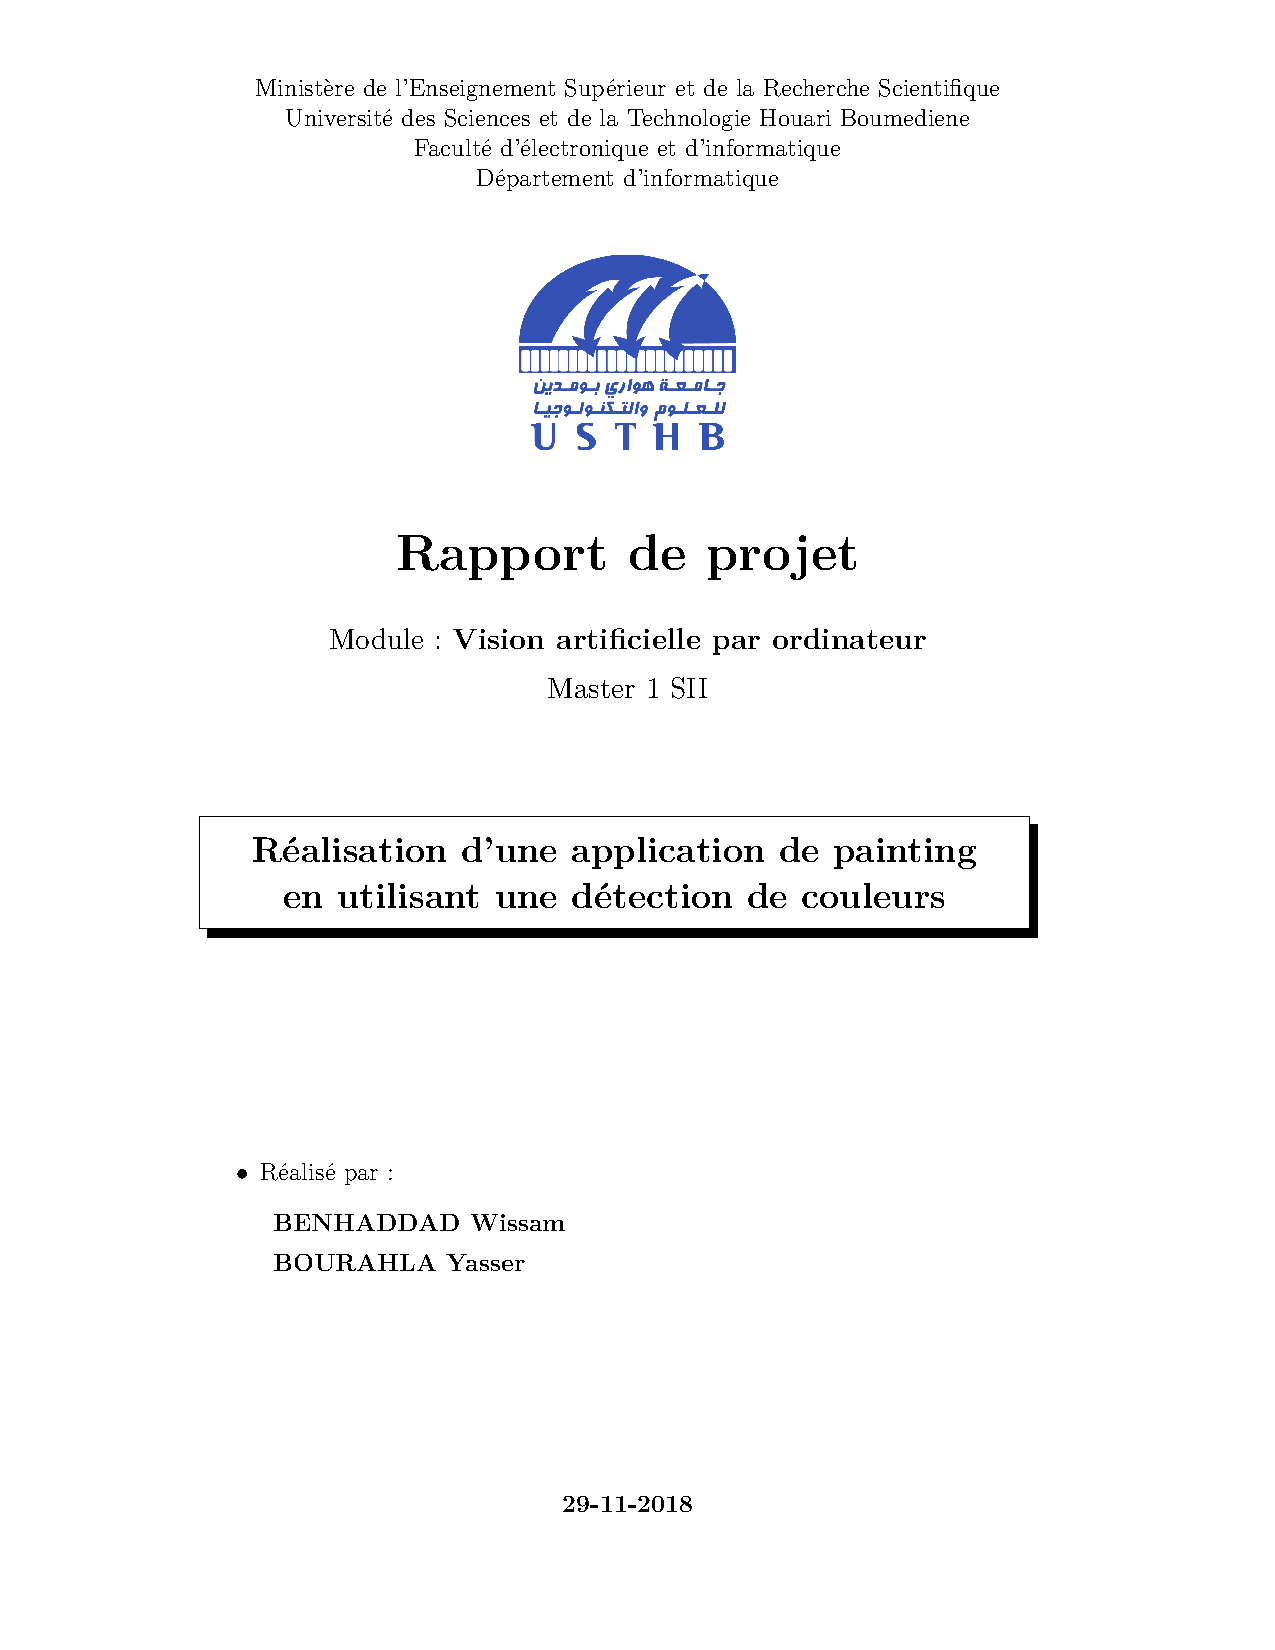
\includepdf[pages=1]{Page_garde.pdf} 
\tableofcontents
\listoffigures
\listoftables


\pagenumbering{arabic}
\newpage
%\title{Réalisation d'un assistant virtuel intelligent pour ordinateurs}
%\author{W.Benhaddad, Y.Bourahla}

\setlist[itemize]{label=\textbullet}
\chapter{Introduction}
\section{Objectifs et problématique}
\paragraph{}
Talk about why we are gonna do this stuff.

\section{Définitions}
\paragraph{}
Some definitions of the concepts,techniques and algorithms that we will use

\subsection{Une image sous différents angles}
\paragraph{}
Talk about how an image can be represented(Color spaces, data structures) BRIEFLY

\subsection{Notion de video}
\paragraph{}
A video is a succession of images at some frame rate, lol

\subsection{Opération sur les images}
\paragraph{}
Notion de filtrage et convolutions

\subsubsection{Filtre moyen}
\subsubsection{Filtre médiane}
\subsubsection{Érosion}
\subsubsection{Dilatation}

NOT SURE IF WE'RE GONNA TALK ABOUT ALL OF THESE ( BAH N3AMROU JEDDOU XD )

\section{Conclusion}

\chapter{Solution proposées et implémentation}

\section{Outils utilisés}

\subsection{Environnement de travail}
\subsection{Langage}
\subsection{OpenCV}
\subsection{Qt framework}

\section{Schéma global du système}
Le système se compose principalement de trois modules:

\begin{itemize}
	\item D’abord le module de détection récupère l’image de la caméra pour y détecter les couleurs recherché et génère des informations sur le curseurs i.e sa position et son état.
	
	\item Le module de dessin reçoit les informations sur le curseur et les utilise pour générer l’image du dessin.
	
	\item Les deux modules précédents envoient leurs résultats à l’interface graphique pour l’affichage.
\end{itemize}

\begin{figure}[H]
	\centering
	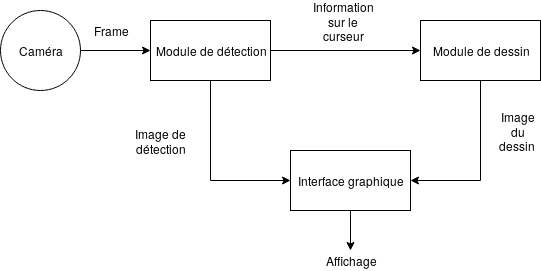
\includegraphics[scale=0.75]{imgs/MainDiagram.png}
	\caption{Schéma du système}
	\label{fig:machineA}
\end{figure}

\section{Détection de couleurs}
La détection de couleurs se fait sur une image en HSV, ceci est dû au fait que HSV sépare la valeur de teinte de celle de la luminosité ce qui le rend plus robuste envers les changements de lumière. 

Ainsi la détection d’une des deux couleur se fait en passant par tous les pixels de l’image et décider pour chaque pixel s’il a la couleur recherché ou non. La décision se fait en testant l’appartenance du pixel à un intervalle de détection. Pour chacune des valeur H,S,V du pixel, on vérifie si cette valeur appartient à un intervalle définit lors du choix de l’utilisateur de la couleur à détecter comme suit: 

Soit la couleur choisie H1S1V1, et le pixel candidat HSV, les conditions que doit vérifier le pixel sont:
\begin{itemize}
	\item $H1-t \leq H \leq H1+t$ : l’intervalle de teinte dépend fortement de la couleur sélectionnée.
	
	\item $S1*0.6 \leq H \leq 255$: l’intervalle de saturation dépend légèrement de la couleur sélectionnée.
	
	\item $20 \leq H \leq 255$: On accepte un intervalle de luminosité large.
\end{itemize}

\section{Élimination du bruit par regroupement}

\section{Conclusion}
Kheliahli rak ta3ref xD 


\chapter{Présentation de l'application}

\section{Diagramme d'utilisation}
\section{Exemples d'utilisation}
\section{Limitations}

\chapter{Conclusion générale}
\paragraph{}



\end{document}}

